%
%
%
% ██╗    ██╗ ██████╗ ██╗████████╗███████╗██╗  ██╗
% ██║    ██║██╔═══██╗██║╚══██╔══╝██╔════╝██║ ██╔╝
% ██║ █╗ ██║██║   ██║██║   ██║   █████╗  █████╔╝
% ██║███╗██║██║   ██║██║   ██║   ██╔══╝  ██╔═██╗
% ╚███╔███╔╝╚██████╔╝██║   ██║   ███████╗██║  ██╗
%  ╚══╝╚══╝  ╚═════╝ ╚═╝   ╚═╝   ╚══════╝╚═╝  ╚═╝
%
%
%
% .##.......####...######..######..##..##.
% .##......##..##....##....##.......####..
% .##......######....##....####......##...
% .##......##..##....##....##.......####..
% .######..##..##....##....######..##..##.
%
%
%
\documentclass[10pt,american]{scrartcl}
\usepackage{amsmath}
\usepackage{amssymb}
\usepackage{babel}
\usepackage{float}
\usepackage[T1]{fontenc}
\usepackage[a4paper]{geometry}
\geometry{tmargin=1.5cm,bmargin=1.5cm,lmargin=1.5cm,rmargin=1.5cm}
\usepackage{graphicx}
\usepackage[none]{hyphenat}
\usepackage[utf8]{inputenc}
\usepackage{microtype}
\pagestyle{empty}
\setlength{\parindent}{0pt}
\setlength{\parskip}{\medskipamount}

\begin{document}

\section*{Sigmoid Function}

\subsection*{Definition}

In the context of Machine Learning, there is a function that appears very
often. We are talking about the \textbf{sigmoid function} $\sigma$. This is the
real function defined as follows:
\begin{equation}
\sigma\left(x\right)=\frac{1}{1+\exp\left(-x\right)},
\label{eq:defn_sigma}
\end{equation}
where $x\in\mathbb{R}$. In these notes, we present the most important results
related to $\sigma$.

\subsection*{Graph}

We begin by taking a look at the graph of the sigmoid function:
\begin{figure}[H]
\centering
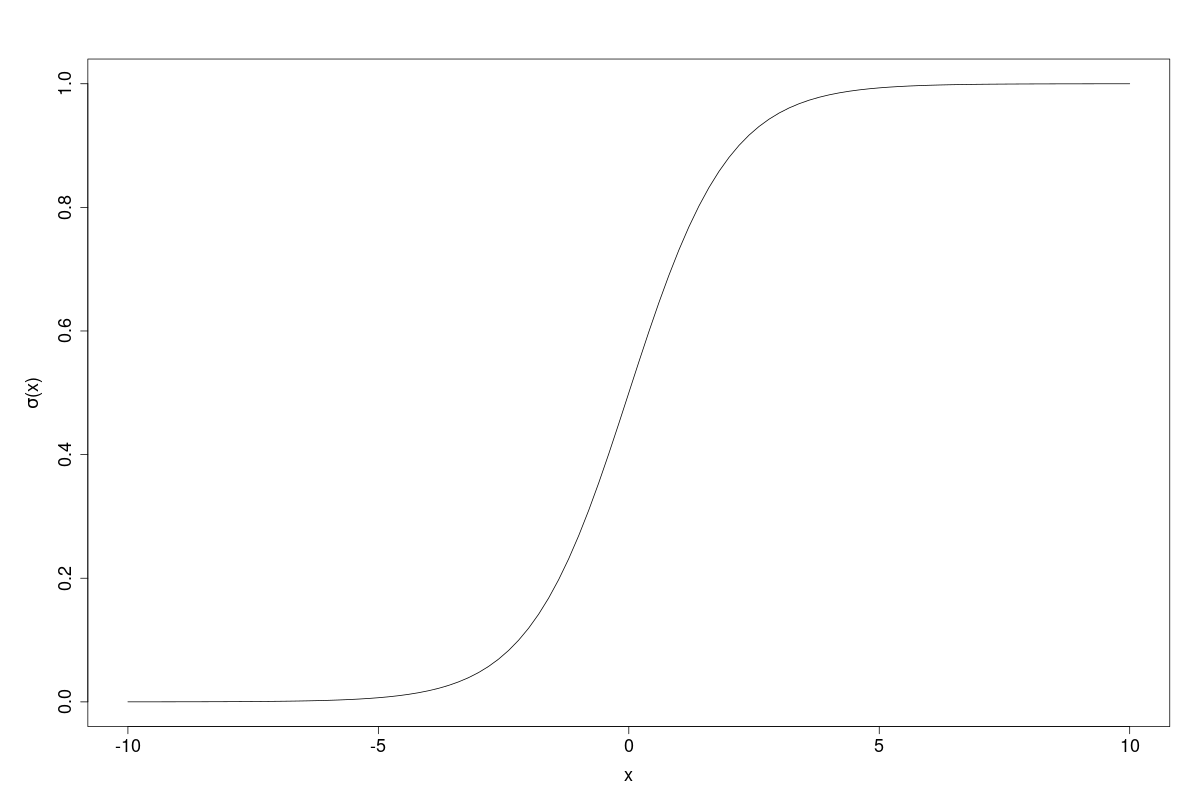
\includegraphics[width=0.7\textwidth]{../r/sigmoid.png}
\caption{Graph of the sigmoid function.}
\label{fig:graph_sigma}
\end{figure}
So essentially $\sigma$ is a function whose curve has a characteristic S-shape.

\subsection*{Boundedness}

Fig.~\ref{fig:graph_sigma} illustrates an important fact: the sigmoid function
is bounded. Specifically, the values returned by $\sigma$ are between 0 and 1.
Next, we prove this fact.

First, consider the lower bound of the sigmoid function. It is well-known that
the exponential function is strictly positive: $\exp\left(x\right)>0$,
$\forall x\in\mathbb{R}$. This allows us to conclude that the denominator on
the RHS of Eq.~(\ref{eq:defn_sigma}) is also strictly positive, i.e.,
$1+\exp\left(-x\right)>0$, $\forall x\in\mathbb{R}$. Hence,
$\sigma\left(x\right)$ is the inverse of a strictly positive real number.
Therefore, we have
\begin{equation}
\sigma\left(x\right)>0,\quad\forall x\in\mathbb{R}.
\label{eq:lower_bound}
\end{equation}

We continue by considering the upper bound of $\sigma\left(x\right)$. Once
again, we use the fact that the exponential function is strictly positive.
This allows us to establish the following inequality:
$1+\exp\left(-x\right)>1$, $\forall x\in\mathbb{R}$. Then the expression on
the RHS of Eq.~(\ref{eq:defn_sigma}) is the inverse of a real number greater
than 1. Hence, the sigmoid function satisfies
\begin{equation}
\sigma\left(x\right)<1,\quad\forall x\in\mathbb{R}.
\label{eq:upper_bound}
\end{equation}

To finish, we combine~(\ref{eq:lower_bound}) and~(\ref{eq:upper_bound}) into a
single inequality, and write
\begin{equation}
0<\sigma\left(x\right)<1,\quad\forall x\in\mathbb{R}.
\label{eq:sigma_bounds}
\end{equation}

\subsection*{Value at the Origin and Special Limits}

By using Eq.~(\ref{eq:defn_sigma}), it is simple to evaluate the sigmoid
function at $x=0$. Since $\exp\left(0\right)=1$, we have
\begin{equation}
\sigma\left(0\right)=\frac{1}{1+\exp\left(0\right)}=\frac{1}{2}.
\label{eq:sigma_at_origin}
\end{equation}

We can also compute the limit of $\sigma\left(x\right)$ as
$x\rightarrow+\infty$. We do so by using the following well-known limit:
\begin{equation*}
\lim_{x\rightarrow+\infty}\exp\left(-x\right)=0.
\end{equation*}
This result allows us to prove that, as $x$ increases arbitrarily, the sigmoid
function approaches 1:
\begin{equation}
\lim_{x\rightarrow+\infty}\sigma\left(x\right)=\frac{1}{1+0}=1.
\end{equation}

Next, we calculate the limit of $\sigma\left(x\right)$ as
$x\rightarrow-\infty$. In this case, we use the following limit of the
exponential function:
\begin{equation*}
\lim_{x\rightarrow-\infty}\exp\left(-x\right)=\infty.
\end{equation*}
Hence, as $x$ decreases arbitrarily, the sigmoid function approaches 0:
\begin{equation}
\lim_{x\rightarrow-\infty}\sigma\left(x\right)=0.
\end{equation}

\subsection*{Relation to the Hyperbolic Tangent}

We proceed by deriving an alternative expression for the sigmoid function.
More precisely, we show how $\sigma\left(x\right)$ can be rewritten in terms of
the hyperbolic tangent. Recall that this function is given by
\begin{equation*}
\tanh\left(x\right)=\frac{\exp\left(x\right)-\exp\left(-x\right)}{\exp\left(x\right)+\exp\left(-x\right)}.
\end{equation*}
Hence:
\begin{equation*}
\tanh\left(\frac{x}{2}\right)=\frac{\exp\left(\frac{x}{2}\right)-\exp\left(-\frac{x}{2}\right)}{\exp\left(\frac{x}{2}\right)+\exp\left(-\frac{x}{2}\right)}.
\end{equation*}
Next, we add 1 to both sides of the above equation:
\begin{align*}
1+\tanh\left(\frac{x}{2}\right)&=\frac{\exp\left(\frac{x}{2}\right)+\exp\left(-\frac{x}{2}\right)}{\exp\left(\frac{x}{2}\right)+\exp\left(-\frac{x}{2}\right)}+\frac{\exp\left(\frac{x}{2}\right)-\exp\left(-\frac{x}{2}\right)}{\exp\left(\frac{x}{2}\right)+\exp\left(-\frac{x}{2}\right)}\\
&=\frac{2\exp\left(\frac{x}{2}\right)}{\exp\left(\frac{x}{2}\right)+\exp\left(-\frac{x}{2}\right)}\\
&=\frac{2}{1+\exp\left(-x\right)}.
\end{align*}
From the last equality, we obtain
\begin{equation}
\sigma\left(x\right)=\frac{1+\tanh\left(\frac{x}{2}\right)}{2}.
\label{eq:sigma_tanh}
\end{equation}

We can use Eq.~(\ref{eq:sigma_tanh}) to establish an interesting property of
the sigmoid function. First, consider $\sigma\left(-x\right)$. Since the
hyperbolic tangent is an odd function, it is simple to prove that
\begin{equation}
\sigma\left(-x\right)=\frac{1-\tanh\left(\frac{x}{2}\right)}{2}.
\label{eq:sigma_minus_tanh}
\end{equation}
Next, we compute the difference $1-\sigma\left(x\right)$. We do so with the
aid of Eq.~(\ref{eq:sigma_tanh}):
\begin{equation}
1-\sigma\left(x\right)=1-\frac{1+\tanh\left(\frac{x}{2}\right)}{2}=\frac{1-\tanh\left(\frac{x}{2}\right)}{2}.
\label{eq:one_minus_sigma}
\end{equation}
Eqs.~(\ref{eq:sigma_minus_tanh}) and~(\ref{eq:one_minus_sigma}) allow us to
write the following identity:
\begin{equation}
\sigma\left(-x\right)=1-\sigma\left(x\right).
\label{eq:sigma_minus}
\end{equation}
We will utilize the above equation to obtain a simple expression for the
derivative of the sigmoid function.

\subsection*{Derivatives}

\subsubsection*{First Derivative}

We begin by stating (without proof) the following: by using simple facts about
analytic functions, it is possible to show that $\sigma\left(x\right)$ is
analytic. This means that the sigmoid function is continuous, and so are all
of its derivatives. Then we can proceed by computing these derivatives.

Let us start by evaluating the first derivative of $\sigma\left(x\right)$. To
do so, we can use the definition of the sigmoid function,
Eq.~(\ref{eq:defn_sigma}). By differentiating both sides of this equation with
respect to $x$, we obtain
\begin{align}
\nonumber\sigma^{\prime}\left(x\right)&=\frac{d}{dx}\left\{\left[1+\exp\left(-x\right)\right]^{-1}\right\}\\
\nonumber&=-\left[1+\exp\left(-x\right)\right]^{-2}\left[-\exp\left(-x\right)\right]\\
&=\frac{\exp\left(-x\right)}{\left[1+\exp\left(-x\right)\right]^{2}}.
\label{eq:sigma_prime_1}
\end{align}

The last result is correct. However, the derivative of the sigmoid function can
be written in a much simpler form in terms of $\sigma\left(x\right)$. Next, we
derive this simpler expression. To do so, we compute the product
$\sigma\left(x\right)\left[1-\sigma\left(x\right)\right]$. First, notice that
Eq.~(\ref{eq:defn_sigma}) allows us to write the following:
\begin{equation*}
1-\sigma\left(x\right)=\frac{\exp\left(-x\right)}{1+\exp\left(-x\right)}.
\end{equation*}
Hence:
\begin{equation}
\sigma\left(x\right)\left[1-\sigma\left(x\right)\right]=\frac{1}{1+\exp\left(-x\right)}\frac{\exp\left(-x\right)}{1+\exp\left(-x\right)}=\frac{\exp\left(-x\right)}{\left[1+\exp\left(-x\right)\right]^{2}}.
\label{eq:product_sigma}
\end{equation}
The last expression is exactly what we have on the RHS of
Eq.~(\ref{eq:sigma_prime_1}). Therefore, we just proved that the derivative of
the sigmoid function can be written as
\begin{equation}
\sigma^{\prime}\left(x\right)=\sigma\left(x\right)\left[1-\sigma\left(x\right)\right].
\label{eq:sigma_prime_2}
\end{equation}
By using Eq.~(\ref{eq:sigma_minus}), we can also express the derivative of
$\sigma\left(x\right)$ as
\begin{equation}
\sigma^{\prime}\left(x\right)=\sigma\left(x\right)\sigma\left(-x\right).
\label{eq:sigma_prime_3}
\end{equation}
This formula makes it very clear that the derivative of the sigmoid function is
even:
\begin{equation*}
\sigma^{\prime}\left(-x\right)=\sigma^{\prime}\left(x\right).
\end{equation*}

We proceed by discussing two important facts about
Eq.~(\ref{eq:sigma_prime_2}). First, we remark that $\sigma\left(x\right)$ is
also known as the \textbf{logistic function}. The function
$\sigma\left(x\right)$ is given this name because the differential equation
\begin{equation*}
\frac{dy\left(x\right)}{dx}=y\left(x\right)\left[1-y\left(x\right)\right]
\end{equation*}
is called the logistic equation. $\sigma\left(x\right)$ is just one of its
particular solutions. Specifically, it is the particular solution that
satisfies $y\left(0\right)=\frac{1}{2}$.

Moreover, Eq.~(\ref{eq:sigma_prime_2}) teaches us something important about the
behavior of the sigmoid function: $\sigma\left(x\right)$ is monotonically
increasing. It is simple to prove this fact with the aid
of~(\ref{eq:sigma_bounds}). According to this inequality, both factors on the
RHS of Eq.~(\ref{eq:sigma_prime_2}) are strictly positive. Hence:
\begin{equation}
\sigma^{\prime}\left(x\right)>0,\quad\forall x\in\mathbb{R}.
\label{eq:pos_der}
\end{equation}
It is also possible to reach this conclusion by analyzing
Eq.~(\ref{eq:sigma_prime_1}). Another confirmation that the
inequality~(\ref{eq:pos_der}) is correct comes from the graph of the derivative
of $\sigma\left(x\right)$ (see Fig.~\ref{fig:graph_sigma_prime}).
\begin{figure}[H]
\centering
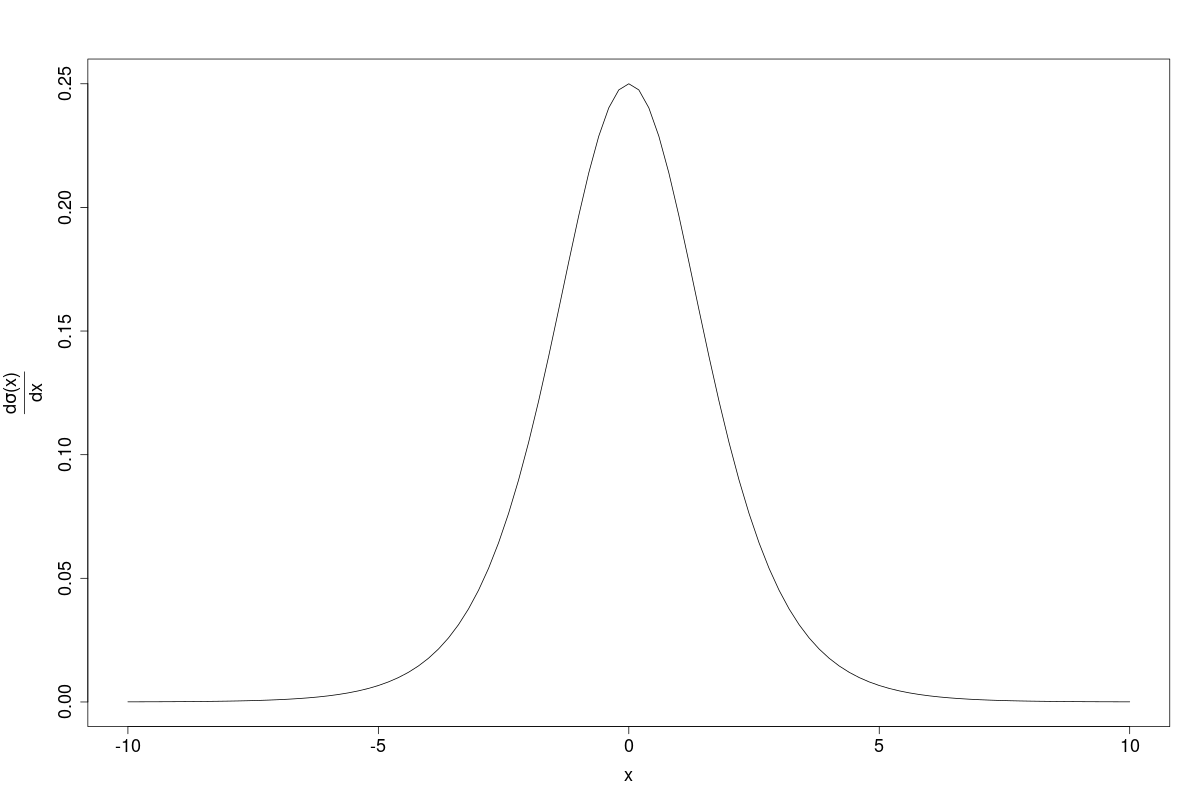
\includegraphics[width=0.7\textwidth]{../r/derivative_sigmoid.png}
\caption{Graph of the first derivative of the sigmoid function.}
\label{fig:graph_sigma_prime}
\end{figure}

To finish this discussion about the first derivative of the sigmoid function,
we derive expressions for $\sigma^{\prime}\left(x\right)$ in terms of
hyperbolic functions. We proceed by using Eq.~(\ref{eq:sigma_prime_3}). Since
we already have formulas for both factors on the RHS of this equation, we can
write
\begin{align}
\nonumber\sigma^{\prime}\left(x\right)&=\sigma\left(x\right)\sigma\left(-x\right)\\
\nonumber&=\frac{1+\tanh\left(\frac{x}{2}\right)}{2}\frac{1-\tanh\left(\frac{x}{2}\right)}{2}\\
\nonumber&=\frac{1-\tanh^{2}\left(\frac{x}{2}\right)}{4}\\
&=\frac{\mathrm{sech}^{2}\left(\frac{x}{2}\right)}{4}.
\end{align}

\subsubsection*{Second Derivative}

To better understand the sigmoid function, we will also compute the second
derivative of $\sigma\left(x\right)$. To do so, we can differentiate both sides
of Eq.~(\ref{eq:sigma_prime_2}) with respect to $x$:
\begin{align}
\nonumber\sigma^{\prime\prime}\left(x\right)&=\frac{d}{dx}\left\{\sigma\left(x\right)\left[1-\sigma\left(x\right)\right]\right\}\\
\nonumber&=\sigma^{\prime}\left(x\right)-2\sigma\left(x\right)\sigma^{\prime}\left(x\right)\\
\nonumber&=\sigma\left(x\right)\left[1-\sigma\left(x\right)\right]\left[1-2\sigma\left(x\right)\right]\\
&=2\sigma^{3}\left(x\right)-3\sigma^{2}\left(x\right)+\sigma\left(x\right).
\label{eq:sigma_sec_der_1}
\end{align}

We can use the above results to show that the sigmoid function has an
inflection point at $x=0$. To establish this fact, we consider the third-degree
polynomial $p$ defined by
\begin{equation}
p\left(x\right)=x\left(1-x\right)\left(1-2x\right)=2x^{3}-3x^{2}+x.
\label{eq:poly_p}
\end{equation}
Clearly, one of the roots of this polynomial is $x=\frac{1}{2}$. By comparing
Eqs.~(\ref{eq:sigma_sec_der_1}) and~(\ref{eq:poly_p}), it is possible to
conclude that the second derivative $\sigma^{\prime\prime}\left(x\right)$
vanishes when the value of $\sigma\left(x\right)$ is $\frac{1}{2}$. According
to Eq.~(\ref{eq:sigma_at_origin}), this happens for $x=0$. Then we just proved
that
\begin{equation}
\sigma^{\prime\prime}\left(0\right)=0.
\label{eq:sec_der_at_origin}
\end{equation}
This is the only situation in which the function
$\sigma^{\prime\prime}\left(x\right)$ vanishes. To understand this statement,
notice that the other two roots of the polynomial $p\left(x\right)$ are $x=0$
and $x=1$. Then the second derivative would also vanish if the sigmoid function
could yield the values 0 and 1. However, according to
Eq.~(\ref{eq:sigma_bounds}), $\sigma\left(x\right)$ returns real numbers
\textit{limited} by these values. Therefore, $x=0$ is the only root of
$\sigma^{\prime\prime}\left(x\right)$.

However, we are not finished. We still have to show that the sign of the second
derivative changes at $x=0$. To do so, we begin by rewriting
$\sigma^{\prime\prime}\left(x\right)$ as follows:
\begin{equation}
\sigma^{\prime\prime}\left(x\right)=\sigma^{\prime}\left(x\right)\left[1-2\sigma\left(x\right)\right].
\label{eq:sigma_sec_der_2}
\end{equation}
We already know that the first factor on the RHS of this equation is always
positive. Then we only need to study the sign of the second factor. Define
$f\left(x\right)=1-2\sigma\left(x\right)$. With the aid of the results we
obtained so far, it is straightforward to establish that this function has the
following properties: (1) $f\left(x\right)$ is monotonically decreasing; (2)
$f\left(x\right)$ vanishes at $x=0$. These properties imply that
$f\left(x\right)<0$ for $x>0$, and $f\left(x\right)>0$ for $x<0$. Since
$f\left(x\right)$ and $\sigma^{\prime\prime}\left(x\right)$ have the same
sign, an analogous statement about $\sigma^{\prime\prime}\left(x\right)$ is
true. Hence, for $x=0$, $\sigma^{\prime\prime}\left(x\right)$ equals zero, and
this function has different signs for positive and negative values of $x$.
This can be seen clearly in the graph of the second derivative,
Fig.~\ref{fig:graph_sec_der_sigma}. Then we have completed our proof that
the sigmoid function has an inflection point at $x=0$.
\begin{figure}[H]
\centering
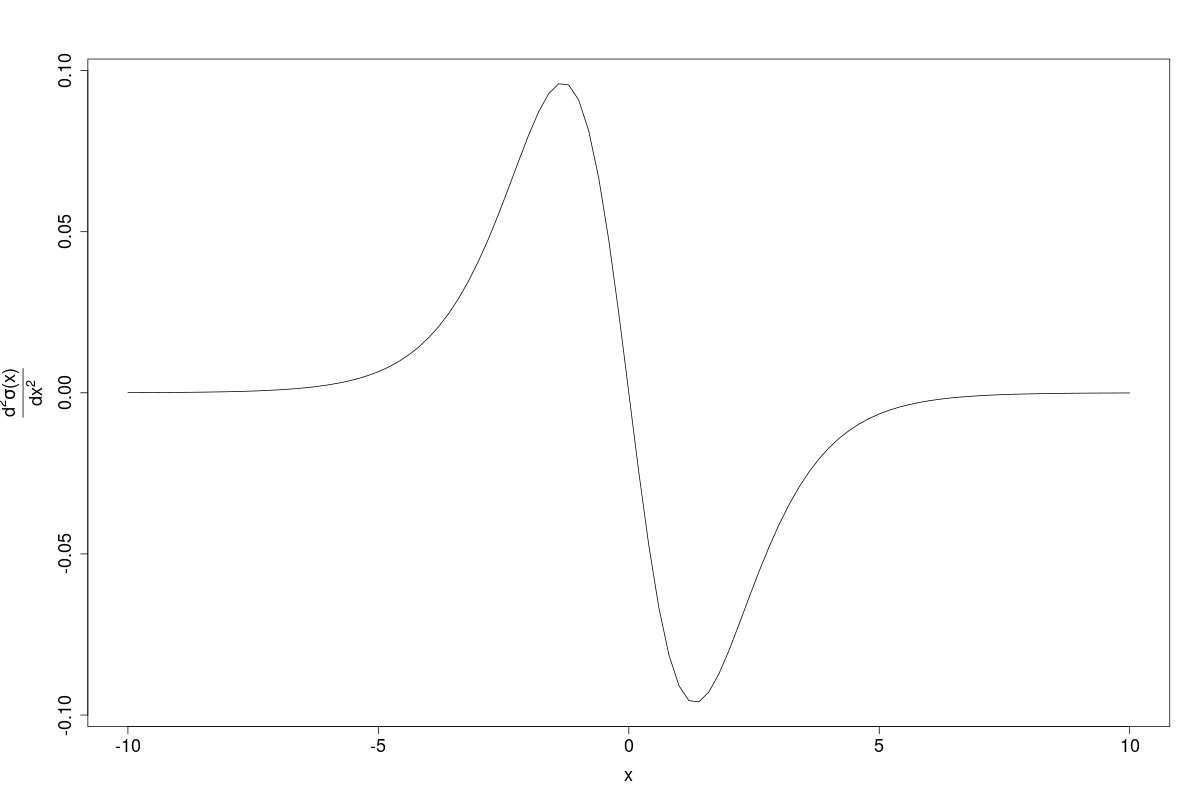
\includegraphics[width=0.7\textwidth]{../r/second_derivative_sigmoid.png}
\caption{Graph of the second derivative of the sigmoid function.}
\label{fig:graph_sec_der_sigma}
\end{figure}

Next, we derive explicit formulas for the second derivative. First, we obtain
an expression in terms of the exponential function. To do so, we can use the
following relation:
$\sigma^{\prime\prime}\left(x\right)=\sigma^{\prime}\left(x\right)f\left(x\right)$.
We already have several equations for the first derivative. Then let us
consider the function $f\left(x\right)$. It can be written as
\begin{align}
\nonumber f\left(x\right)&=1-2\sigma\left(x\right)\\
\nonumber&=1-\frac{2}{1+\exp\left(-x\right)}\\
&=\frac{\exp\left(-x\right)-1}{1+\exp\left(-x\right)}.
\end{align}
To continue, we multiply the last result by $\sigma^{\prime}\left(x\right)$:
\begin{align}
\nonumber\sigma^{\prime\prime}\left(x\right)&=\sigma^{\prime}\left(x\right)f\left(x\right)\\
\nonumber&=\frac{\exp\left(-x\right)}{\left[1+\exp\left(-x\right)\right]^{2}}\frac{\exp\left(-x\right)-1}{1+\exp\left(-x\right)}\\
&=\frac{\exp\left(-x\right)\left[\exp\left(-x\right)-1\right]}{\left[1+\exp\left(-x\right)\right]^{3}}.
\end{align}

We can follow an analogous procedure to express the second derivative in terms
of hyperbolic functions. We begin by rewriting the function $f\left(x\right)$.
With the aid of Eq.~(\ref{eq:sigma_tanh}), it is possible to write
\begin{align}
\nonumber f\left(x\right)&=1-2\sigma\left(x\right)\\
\nonumber&=1-1-\tanh\left(\frac{x}{2}\right)\\
&=-\tanh\left(\frac{x}{2}\right).
\end{align}
Notice that the last equality shows that $f\left(x\right)$ is an odd function.
We already established that the first derivative
$\sigma^{\prime}\left(x\right)$ is even. These facts allow us to conclude that
the second derivative $\sigma^{\prime\prime}\left(x\right)$ is odd.
To complete our derivation, we only need to multiply the above expression by
our result for $\sigma^{\prime}\left(x\right)$ in terms of the hyperbolic
secant:
\begin{align}
\nonumber\sigma^{\prime\prime}\left(x\right)&=\sigma^{\prime}\left(x\right)f\left(x\right)\\
\nonumber&=\frac{\mathrm{sech}^{2}\left(\frac{x}{2}\right)}{4}\left[-\tanh\left(\frac{x}{2}\right)\right]\\
&=-\frac{\tanh\left(\frac{x}{2}\right)\mathrm{sech}^{2}\left(\frac{x}{2}\right)}{4}.
\end{align}

\end{document}
